%!TEX root = skripsi.tex
%-----------------------------------------------------------------------------%
\chapter{\babEmpat} \label{eksperimen}
%-----------------------------------------------------------------------------%

\section{Normalisasi Data}
Data yang sudah diperoleh perlu dinormalisasi terlebih dahulu untuk membuang \f{noise} yang dapat mengganggu jalannya eksperimen. Normalisasi dilakukan dengan cara membuang suara senyap atau \f{silence}. Ada beberapa teknik yang digunakan untuk membuang \f{silence}. Salah satu teknik klasik dan populer yang digunakan untuk membuang \f{silence} pada suara adalah kombinasi \f{short term energy} (STE) dengan \f{zero crossing rate} (ZCR) \citep{rabiner1978digital}. \cite{saha2005new} memaparkan pendekatan lain yang lebih baik akurasinya dalam membuang \f{silence} jika dibandingkan dengan STE maupun kombinasi ZCR dengan STE, yaitu dengan memodelkan sinyal audio menggunakan distribusi \f{Gaussian}.

Penelitian ini menggunakan pendekatan yang dipaparkan oleh \cite{saha2005new} dalam membuang \f{silence}, dengan langkah-langkah sebagai berikut.

\begin{enumerate}
	\item \label{satu} Hitung rata-rata ($\mu$) dan standar deviasi ($\sigma$) dari 10 ms sampel pertama pada audio. Jika $fs$ menyatakan \br~dari audio, maka terdapat sebanyak $s$ sampel dalam 10 ms.
	\begin{align}
    s &= 0.01\cdot fs \\
		\mu &= \frac{\sum_{i=1}^{s}x(i)}{s} \\
		\sigma &= \sqrt{\frac{\sum_{i=1}^{s}(x(i)-\mu)^2}{s}}
	\end{align}
	\f{Background noise} juga dikenali dari berdasarkan nilai rata-rata ($\mu$) dan standar deviasinya ($\sigma$).

	\item Periksa apakah jarak \f{Mahalanobis} mulai dari sampel pertama sampai dengan sampel terakhir pada audio lebih dari $3$ atau tidak. Jarak \f{Mahalanobis} dihitung menggunakan fungsi $f$ sebagai berikut.
	\begin{equation}
		d(x) = \frac{|x-\mu|}{\sigma}
	\end{equation}
	Nilai $3$ dipilih karena pada distribusi \f{Gaussian}, 99.7\% data memiliki nilai jarak \f{Mahalanobis} $\leq3$. Gambar \ref{fig:distribusinormal} menunjukkan persebaran data pada distribusi \f{Gaussian}.

	\begin{figure}
		\centering
		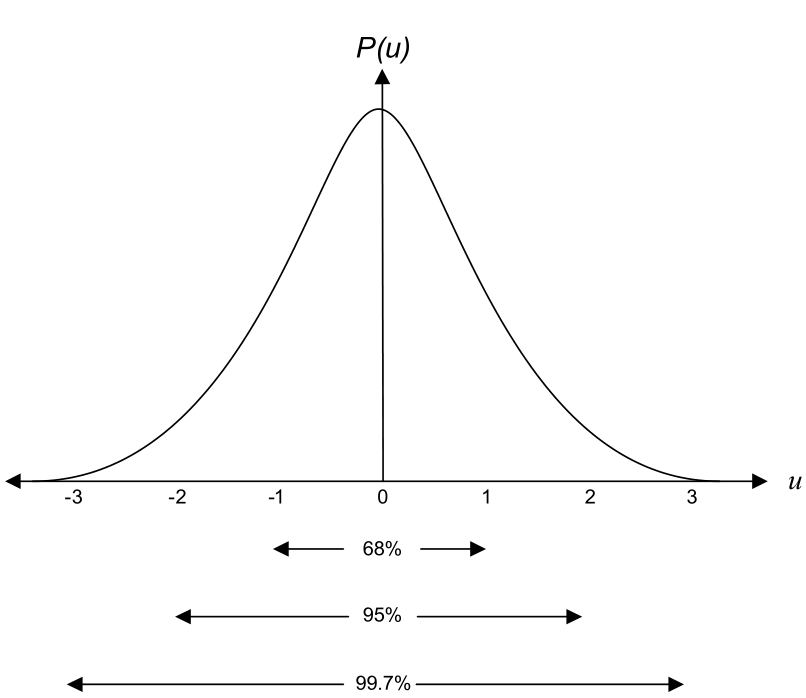
\includegraphics[width=0.85\linewidth]{pics/distribusi_normal}
		\caption{Distribusi \f{Gaussian} Terhadap Nilai Jarak \f{Mahalanobis}}{Sumber gambar: \cite{saha2005new}}
		\label{fig:distribusinormal}
	\end{figure}

	\item Tandai sampel yang dianggap bukan sebagai \f{silence} (selanjutnya disebut \f{voiced}) dengan 1 dan sampel yang dianggap sebagai \f{silence} dengan 0. Bagi keseluruhan sinyal audio ke dalam beberapa bagian yang tidak saling \f{overlap}, dengan durasi pada setiap bagian adalah 10 ms.

	\item \label{empat} Asumsikan ada $M$ sampel yang bernilai 0 dan $N$ sampel yang bernilai 1. Jika $M \geq N$, maka ubah setiap tanda 1 menjadi tanda 0, dan sebaliknya.

	\item Kumpulkan seluruh bagian yang dianggap sebagai \f{voiced}, yaitu bagian-bagian yang bertanda 1 hasil dari langkah \ref{satu} sampai langkah \ref{empat}.
\end{enumerate}


	
\section{Ekstraksi Fitur} \label{chap:ekstraksi fitur}
Ekstraksi fitur adalah proses mengubah data \f{input} menjadi himpunan fitur-fitur yang dapat merepresentasikan data \f{input} dengan baik. Ekstraksi fitur merupakan bentuk istimewa dari \f{dimensionality reduction} \citep{Soft-Computational}. \cite{wyse1980critical} menjelaskan bahwa ekstraksi fitur adalah proses yang mengekstrak himpunan fitur-fitur baru dari fitur asli melalui serangkaian fungsi pemetaan. Penelitian ini menggunakan dua jenis fitur, yaitu \f{mel frequency cepstral coefficient} (MFCC) dan \f{shifted delta cepstral coefficient} (SDCC). Fitur MFCC dipilih karena MFCC merupakan fitur yang banyak digunakan dalam penelitian di bidang \f{speech recognition} \citep{young2002htk}. Contohnya adalah penelitian yang berjudul \f{Voice Content Matching System for Quran Readers} oleh \cite{Muhammad:2010:VCM:1934908.1935467}. Sedangkan fitur SDCC dipilih karena SDCC merupakan fitur yang memuat lebih banyak konteks dalam setiap \f{frame}-nya jika dibandingkan dengan MFCC.

% Data jenis mp3 terlalu kompleks untuk diklasifikasi secara langsung menggunakan metode-metode yang ada saat ini. Selain itu, banyak informasi tidak perlu atau \f{noise} yang terdapat pada sebuah berkas mp3. Untuk itu diperlukan proses ekstraksi fitur. Dengan proses ini diharapkan hanya informasi penting saja yang terambil dari sebuah berkas mp3 dan memiliki bentuk yang tidak terlalu kompleks.

\subsection{Ekstraksi Fitur MFCC} \label{chap:ekstrak fitur mfcc}
Ekstraksi fitur MFCC menggunakan fungsi \f{mfcc} yang telah dijelaskan di Bab \ref{chap:fungsipendukung}. Fungsi \f{mfcc} pada eksperimen ini dipanggil dengan parameter fungsi yang dijelaskan pada tabel \ref{table:pemanggilanmfcc}.
\begin{table}
	\centering
  \caption{Parameter Pemanggilan Fungsi \f{mfcc}}
  \begin{tabular}{|l|l|}
    % mfcc( speech, fs, Tw, Ts, alpha, window, R, M, N, L )
    \hline
    \textbf{Nama Parameter} & \textbf{Nilai Parameter} \\ \hline
    Tw & 25 ms \\ \hline
    Ts & 10 ms \\ \hline
    Alpha & 0.97 \\ \hline
    Window & \f{hamming window}  \\ \hline
    R & [300 3700] \\ \hline
    M & 20 \\ \hline
    C & 13 \\ \hline
    L & 22 \\ \hline
  \end{tabular}
  \label{table:pemanggilanmfcc}
 \end{table}

Berikut adalah langkah-langkah untuk memproses fitur MFCC.
\begin{enumerate}
  \item Tentukan nilai \br~untuk dimasukkan dalam perhitungan MFCC, yang akan mempengaruhi durasi audio. Durasi sebuah audio (dalam detik), $d$, dapat dihitung dengan rumus
  \begin{equation}
    d = \frac{L}{fs}, 
  \end{equation}
  di mana $L$ adalah panjang \fr~audio dan $fs$ adalah \br. Banyaknya \fr~(panjang kolom) pada hasil ekstraksi nilai MFCC dipengaruhi oleh durasi audionya. Maka untuk menyamakan panjang kolom hasil ekstraksi MFCC, durasi audio-audio yang akan diproses harus disamakan terlebih dahulu. Durasi yang digunakan untuk mengekstrak nilai MFCC pada satu ayat tertentu adalah \f{nilai rata-rata durasi} keseluruhan audio dari berbagai qari pada ayat tersebut. Setelah diperoleh nilai rata-rata durasi, $\bar{d}$, langkah selanjutnya adalah membuat masing-masing audio memiliki durasi yang sama, dengan cara mengubah nilai $fs$ masing-masing audio. Jika diberikan nilai $\bar{d}$ dan $L$, maka nilai $fs$ yang baru, $\widehat{fs}$, dihitung menggunakan rumus
  \begin{equation}
    \widehat{fs} = \frac{L}{\bar{d}}.
  \end{equation}


	\item Panggil fungsi \f{mfcc} dengan parameter yang telah disebutkan pada tabel \ref{table:pemanggilanmfcc} dan nilai \br~sama dengan $\widehat{fs}$, sehingga memberikan \f{output} berupa matriks MFCC 13x$K$, di mana $K$ menyatakan banyaknya \fr.

	\item Buang matriks MFCC pada baris pertama, karena nilai tersebut merupakan log energi yang bukan merupakan bagian dari fitur dalam eksperimen ini. Sehingga matriks MFCC yang tersisa berukuran $12\times K$.

	\item Hitung nilai rata-rata pada setiap \fr~matriks MFCC. Perhitungan tersebut akan menghasilkan vektor kolom, $\vec v$, dengan panjang $K$. Vektor kolom adalah matriks yang hanya memiliki satu baris.

	\item Selanjutnya vektor tersebut dipendekkan dengan cara sebagai berikut.
	\begin{enumerate}[label*=\arabic*.]
		\item Tentukan nilai $s$ (\f{shift}). $s = \left\lceil\frac{K}{30}\right\rceil$.
		\item Tentukan nilai $w$ (\f{width}). $w = \left\lceil1.5 \times s\right\rceil$.
		\item Setiap $s$ elemen sekali, hitung nilai rata-rata dari $w$ elemen berurutan pada vektor $\vec{v}$.
	\end{enumerate}
	Hasil pemendekan tersebut berupa vektor $\widehat{\vec{v}}$ dengan panjang $\widehat K$, di mana \[ \widehat{K} = \left\lceil \frac{K-w+1}{s} \right\rceil = \left\lceil \frac{K-1.5\left\lceil\frac{K}{30}\right\rceil+1}{\left\lceil\frac{K}{30}\right\rceil} \right\rceil \leq 29. \] Tujuan dari pemendekan vektor ini adalah untuk mengurangi kompleksitas fitur sehingga diharapkan hasil klasifikasi akan lebih akurat.
  
  Gambar \ref{fig:alurekstraksifiturmfcc} menunjukkan alur proses ekstraksi fitur MFCC.
  \begin{figure}
    \centering
    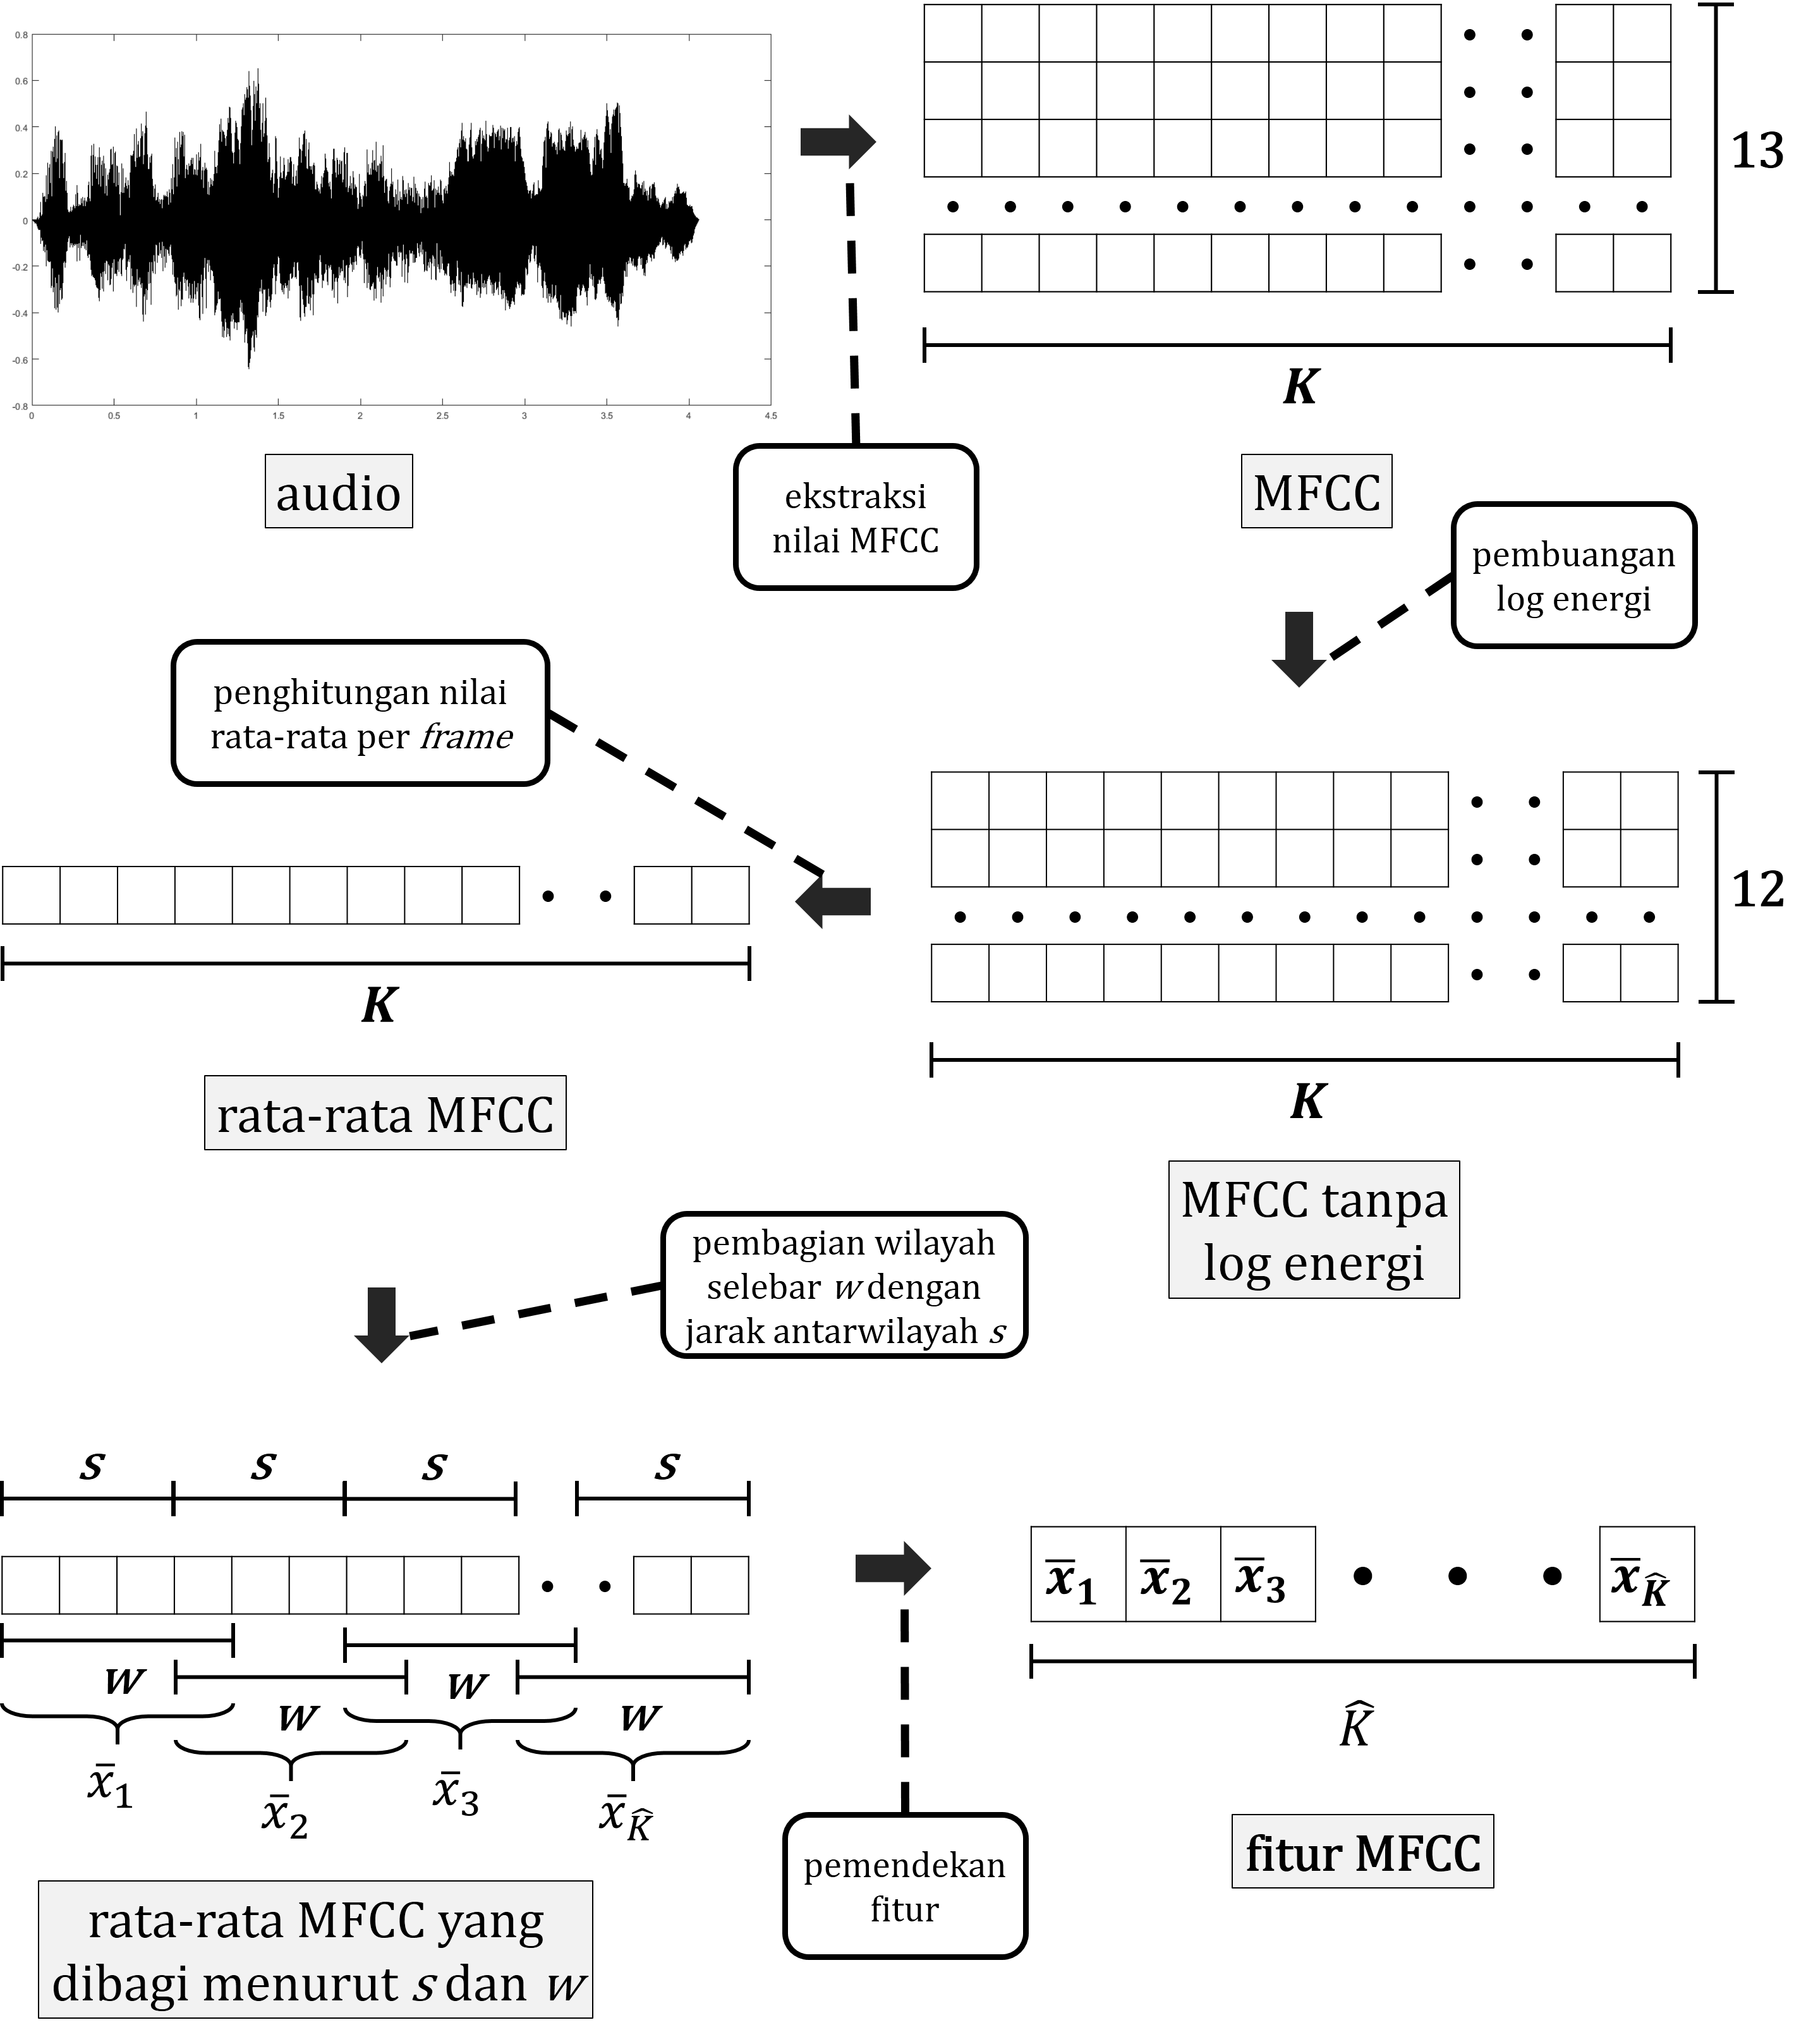
\includegraphics[width=\linewidth]{pics/ekstraksi_mfcc_v3}
    \caption{Alur Ekstraksi Fitur MFCC}
    \label{fig:alurekstraksifiturmfcc}
  \end{figure}
\end{enumerate}



\subsection{Ekstraksi Fitur SDCC}
Ekstraksi fitur SDCC menggunakan fungsi \f{mfcc2sdc} yang telah dijelaskan di Bab \ref{chap:fungsipendukung}. Fungsi \f{mfcc2sdc} pada eksperimen ini dipanggil dengan parameter fungsi yang dijelaskan pada tabel \ref{table:pemanggilansdcc}.
\begin{table}
	\centering
  \caption{Parameter Pemanggilan Fungsi \f{mfcc2sdc}}
  \begin{tabular}{|l|l|}
    % mfcc2sdc(CepCoeff,d,P,K)
    \hline
    \textbf{Nama Parameter} & \textbf{Nilai Parameter} \\ \hline
    D (nilai \f{shift} untuk \f{delta computation}) & 1 \\ \hline
    P (nilai \f{shift} untuk \fr~selanjutnya) & 3 \\ \hline
    K (banyaknya blok di mana koefisien \f{delta} disambungkan) & 3 \\ \hline
  \end{tabular}
  \label{table:pemanggilansdcc}
 \end{table}

Berikut adalah langkah-langkah untuk memproses fitur SDCC.
\begin{enumerate}
  \item Hitung nilai MFCC menggunakan fungsi \f{mfcc} seperti sudah dijelaskan di Bab \ref{chap:ekstrak fitur mfcc}, langkah 1 sampai 3, sehingga diperoleh nilai MFCC berupa matriks berukuran $12\times K$. Nilai MFCC berukuran $12\times K$ perlu di-\f{transpose} terlebih dahulu menjadi ukuran $K\times12$ untuk menyesuaikan kebutuhan fungsi \f{mfcc2sdc}, yaitu baris sebagai \fr~dan kolom sebagai koefisien.

	\item Panggil fungsi \f{mfcc2sdc} dengan parameter yang telah disebutkan pada tabel \ref{table:pemanggilansdcc}, sehingga memberikan \f{output} berupa matriks SDCC $36\times L$, di mana $L$ menyatakan banyaknya \fr.

	\item Hitung nilai rata-rata pada setiap \fr~matriks SDCC. Perhitungan tersebut akan menghasilkan vektor kolom, $w$, dengan panjang $L$.

	\item Selanjutnya vektor tersebut dipendekkan dengan cara sebagai berikut.
	\begin{enumerate}[label*=\arabic*.]
		\item Tentukan nilai $s$ (\f{shift}). $s = \left\lceil\frac{L}{30}\right\rceil$.
		\item Tentukan nilai $w$ (\f{width}). $w = \left\lceil1.5\times s\right\rceil$.
		\item Setiap $s$ elemen sekali, hitung nilai rata-rata dari $w$ elemen berurutan pada vektor $\vec{w}$.
	\end{enumerate}
	Hasil pemendekan tersebut berupa vektor $\widehat{\vec{w}}$ dengan panjang $\widehat L$, di mana \[ \widehat L = \left\lceil \frac{L-w+1}{s} \right\rceil = \left\lceil \frac{L-1.5\left\lceil\frac{L}{30}\right\rceil+1}{\left\lceil\frac{L}{30}\right\rceil} \right\rceil \leq 29. \] Tujuan dari pemendekan vektor ini adalah untuk mengurangi kompleksitas fitur sehingga diharapkan hasil klasifikasi akan lebih akurat.

  Gambar \ref{fig:alurekstraksifitursdcc} menunjukkan alur proses ekstraksi fitur SDCC.
  \begin{figure}
    \centering
    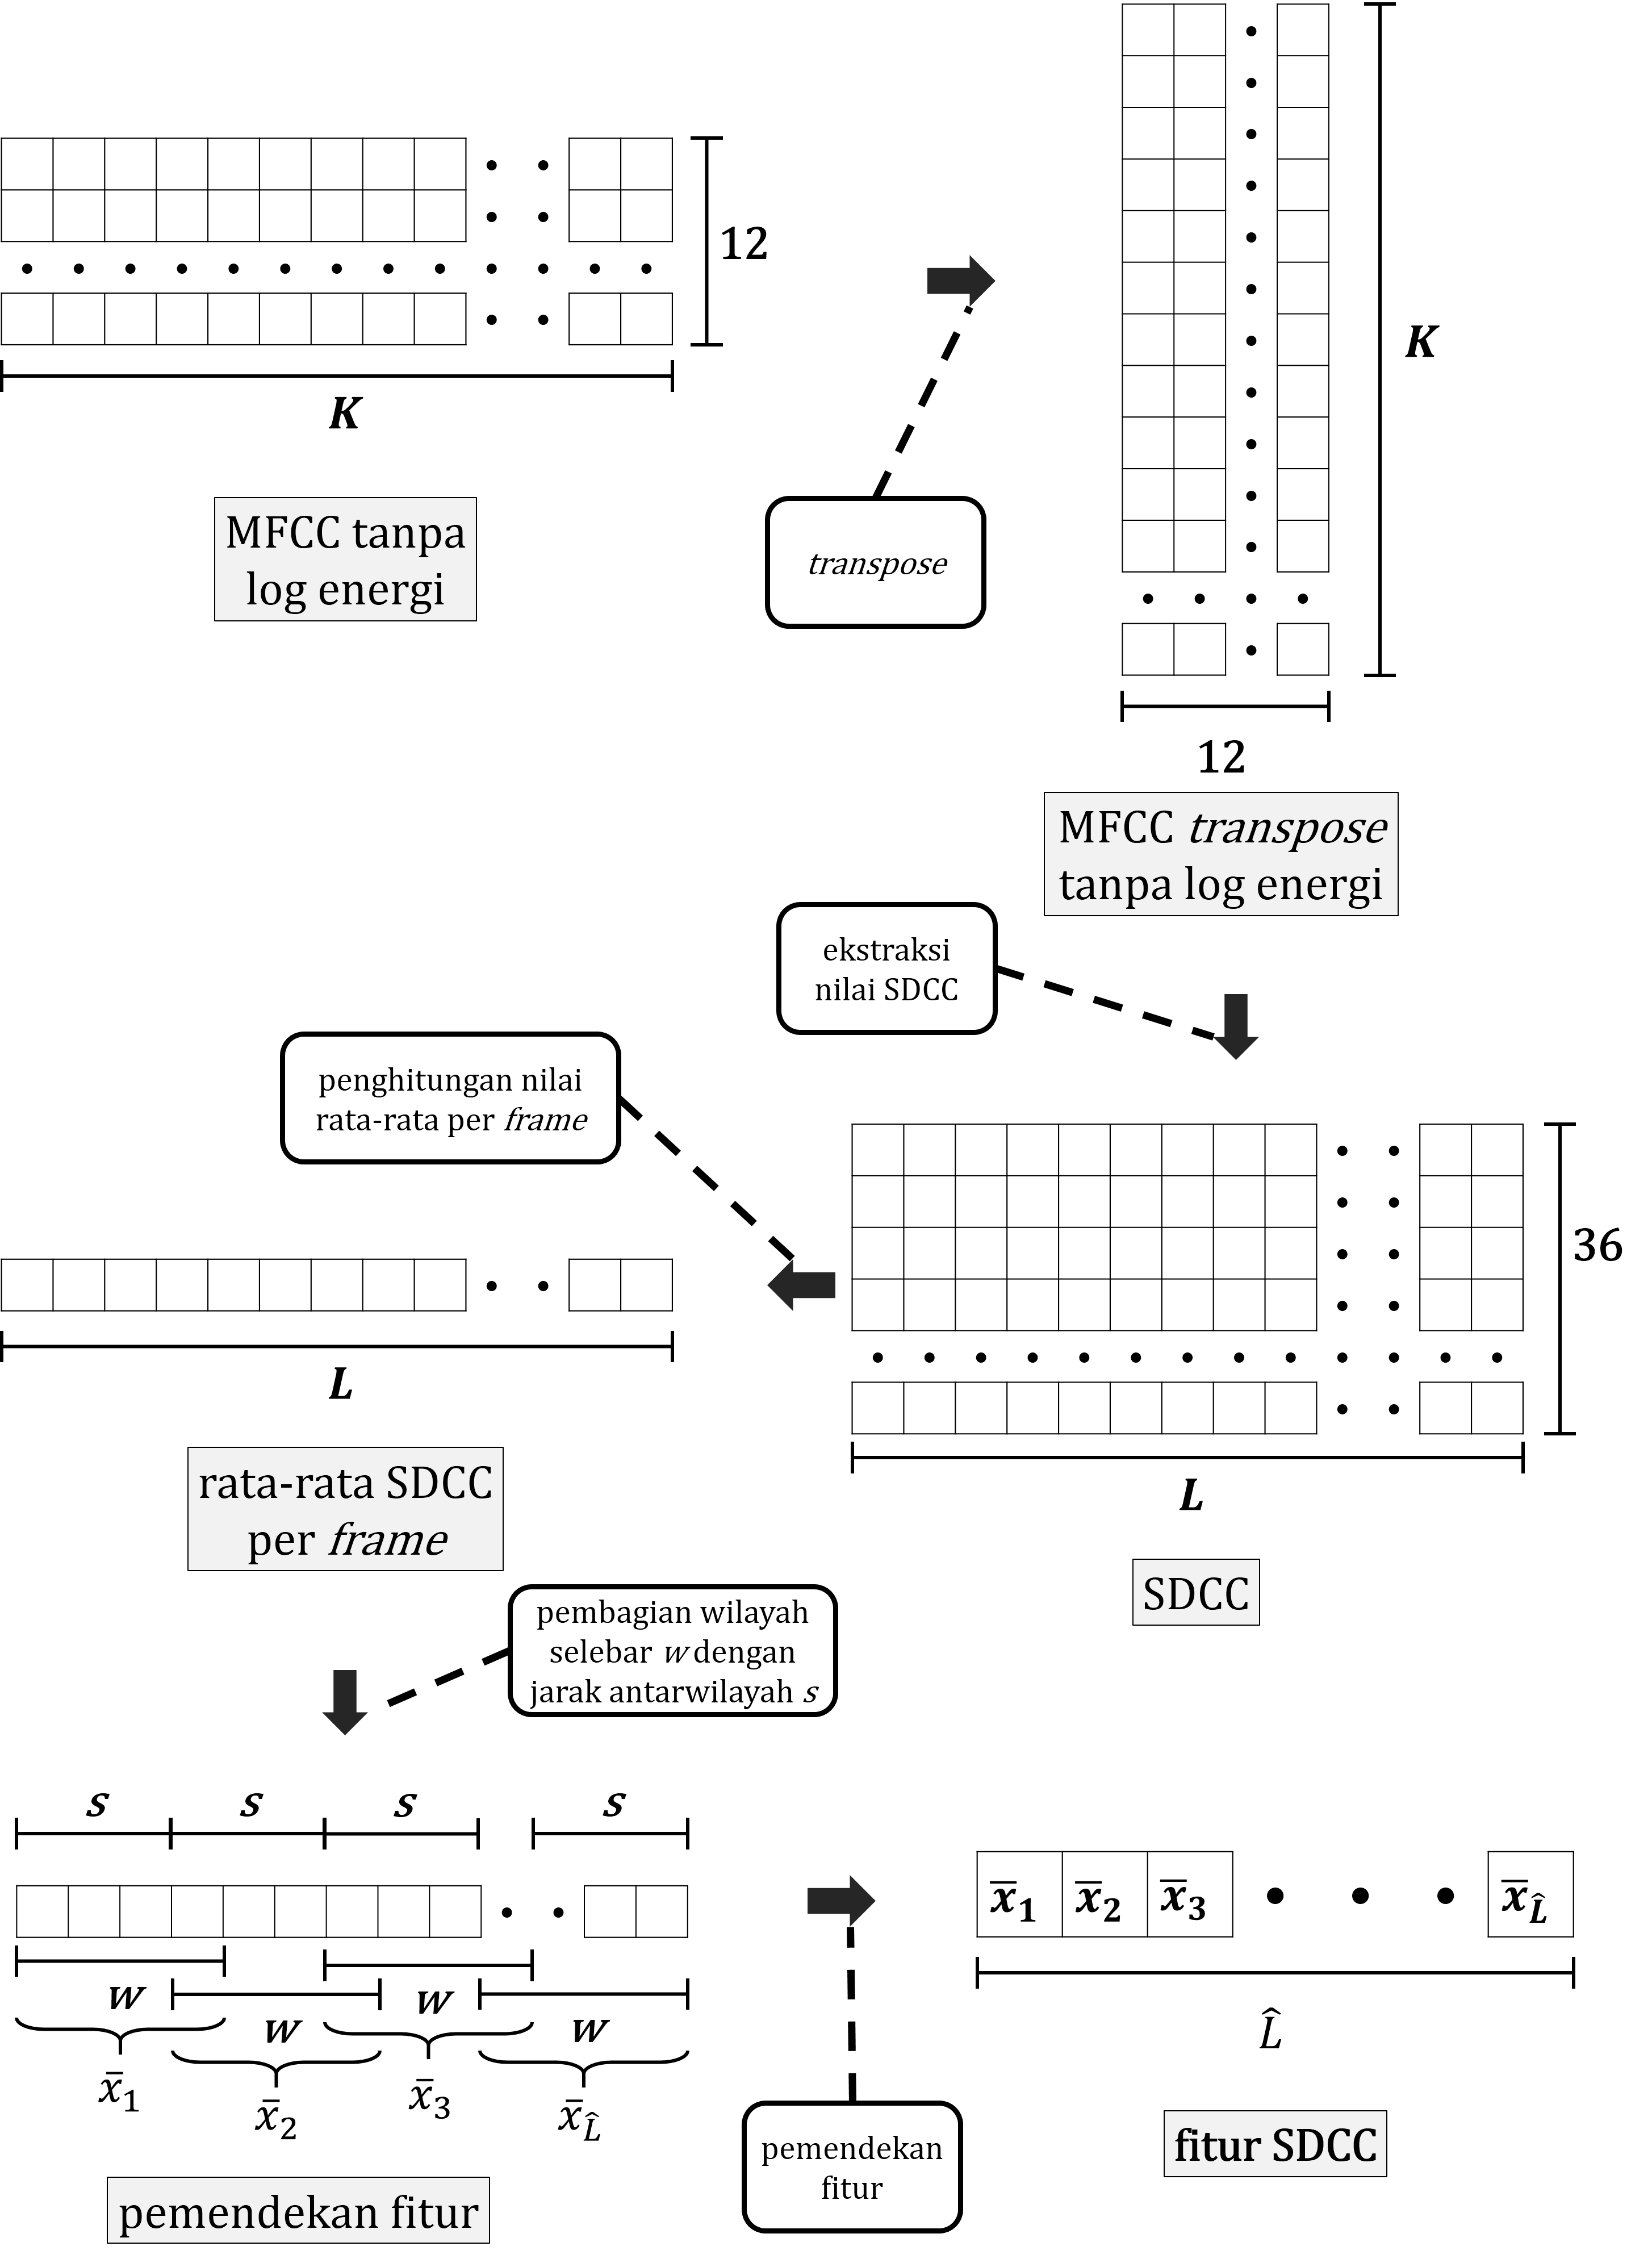
\includegraphics[width=\linewidth]{pics/ekstraksi_sdcc_v2}
    \caption{Alur Ekstraksi Fitur SDCC}
    \label{fig:alurekstraksifitursdcc}
  \end{figure}
\end{enumerate}



\section{Pemodelan} \label{chap:pemodelan}
Penelitian ini menggunakan tiga variasi metode klasifikasi untuk mengenali pola dari fitur-fitur yang dihasilkan melalui proses pada Bab \ref{chap:ekstraksi fitur}, yaitu \f{support vector machine} (SVM), \f{Gaussian mixture model} (GMM), serta gabungan SVM dengan GMM. SVM dipilih untuk digunakan dalam penelitian ini karena SVM merupakan metode klasifikasi biner yang \f{powerful} \citep{bishop2006pattern}. Sedangkan GMM dipilih untuk digunakan dalam penelitian ini karena GMM merupakan model yang banyak digunakan dalam penelitian di bidang \f{speaker verification} \citep{reynolds2000speaker} dan \f{language identification} \citep{torres2002approaches}, serta sudah menjadi salah satu pendekatan terbaik dalam kedua bidang tersebut \citep{zahra2013unique}.

Satu ayat dari berbagai qari dimodelkan menjadi sebuah model klasifikasi. Ayat-ayat yang sama dari para qari akan dijadikan data sampel dengan label \f{benar}. Ayat-ayat selain ayat tersebut yang tidak mirip secara tekstual akan dijadikan data sampel dengan label \f{salah}. Cara mengetahui dua buat ayat mirip secara tekstual adalah menggunakan pendekatan algoritma \f{dynamic programming} yang sudah dijelaskan pada Bab \ref{lcs}.

	\subsection{Pemodelan dengan Support Vector Machine (SVM)}
	SVM dipilih untuk digunakan dalam eksperimen ini karena memiliki kemampuan yang terbukti kuat dalam melakukan klasifikasi pola. Hal tersebut dijelaskan oleh \cite{campbell2006support} dalam jurnalnya yang berjudul \f{Support Vector Machines for Speaker and Language Recognition}. SVM didasari oleh teori-teori matematika yang kuat, antara lain dengan adalah pemetaan data ke dimensi ruang yang lebih tinggi, pencarian \f{margin} terbesar, dan generalisasi. Alasan lain yang memperkuat penggunaan SVM dalam penelitian ini adalah karena SVM merupakan metode klasifikasi dua kelas, sesuai dengan kebutuhan sistem untuk mengklasifikasi data ke dalam dua kelas, yaitu kelas \f{benar} dan kelas \f{salah}.

  Metode klasifikasi SVM dalam eksperimen ini menggunakan fungsi MATLAB \f{svmtrain}\footnote{http://www.mathworks.com/help/stats/svmtrain.html} dalam proses pemodelan dan \f{svmclassify}\footnote{http://www.mathworks.com/help/stats/svmclassify.html} dalam proses pengujian, dengan parameter yang dijelaskan pada Tabel \ref{table:parametersvm} berikut.

  \begin{table}
    \centering
    \caption{Parameter SVM dalam Eksperimen}
    \begin{tabular}{|c|c|}
      \hline
      \textbf{Nama Parameter} & \textbf{Nilai Parameter} \\ \hline
      kernel\_function & linear \\ \hline
      method & Sequential Minimal Optimization (SMO) \\ \hline
      MaxIter & 15000 \\ \hline
    \end{tabular}
    \label{table:parametersvm}
  \end{table}



  \subsection{Pemodelan dengan Gaussian Mixture Model (GMM)}
  GMM dipilih dalam eksperimen ini karena banyak penelitian yang menyatakan bahwa GMM dapat memodelkan fitur-fitur \f{speech recognition} dengan baik, salah satunya adalah penelitian yang dilakukan oleh \cite{zahra2013unique}. Ayat-ayat yang berlabel \f{benar} dimodelkan menjadi sebuah GMM, sedangkan ayat-ayat yang berlabel \f{salah} dimodelkan menjadi sebuah GMM lain, sehingga untuk satu ayat terdapat dua GMM yang menjadi model dalam melakukan klasifikasi. Cara menentukan apakah satu data uji masuk ke dalam kelas \f{benar} atau \f{salah} adalah dengan membandingkan nilai PDF dari kedua model tersebut. Jika nilai PDF pada GMM yang memodelkan kelas \f{benar} lebih besar atau sama dengan nilai PDF pada GMM yang memodelkan kelas \f{salah}, maka data uji tersebut diklasifikasikan sebagai data \f{benar}. Selain itu maka data uji tersebut diklasifikasikan sebagai data \f{salah}.

  Metode klasifikasi GMM dalam eksperimen ini menggunakan fungsi MATLAB \f{gmdistribution.fit}\footnote{http://www.mathworks.com/help/stats/gmdistribution.fit.html} dalam proses pemodelan dengan parameter yang dijelaskan pada Tabel \ref{table:parametergmm} berikut.

  \begin{table}
    \centering
    \caption{Parameter GMM dalam Eksperimen}
    \begin{tabular}{|c|c|}
      \hline
      \textbf{Nama Parameter} & \textbf{Nilai Parameter} \\ \hline
      k & 8 \\ \hline
      CovType & diagonal \\ \hline
      SharedCov & true \\ \hline
      MaxIter & 100 \\ \hline
    \end{tabular}
    \label{table:parametergmm}
  \end{table}



  \subsection{Pemodelan dengan Gabungan SVM dan GMM}
	Kemampuan SVM maupun GMM untuk menjadi model sistem ASR sudah teruji baik oleh beberapa penelitian \citep{zahra2013unique}. Maka dalam eksperimen ini dicoba pula gabungan dari dua metode klasifikasi tersebut. Cara menggabungkan dua metode tersebut dalam proses pemodelan adalah sebagai berikut.
	\begin{enumerate}
    \item Buat model pertama, $M_{SVM}$ menggunakan metode klasifikasi SVM dan data sampel.
    \item Buat model kedua, $M_0$ menggunakan GMM dengan sampel data berlabel \f{salah} dan data sampel.
    \item Buat model ketiga, $M_1$ menggunakan GMM dengan sampel data berlabel \f{benar} dan data sampel.
  \end{enumerate}
  Sedangkan cara menggabungkan dua metode tersebut dalam proses pengujian adalah sebagai berikut.
  \begin{enumerate}
    \item Hitung nilai PDF dari data uji pada $M_0$, $P_0$, sebagai nilai probabilitas \f{salah}.
    \item Hitung nilai PDF dari data uji pada $M_1$, $P_1$, sebagai nilai probabilitas \f{benar}.
    \item Klasifikasikan data uji menggunakan metode klasifikasi SVM. dengan model $M_{SVM}$ Jika hasil klasifikasinya bernilai \f{salah}, tambahkan nilai 1 pada $P_0$, dan jika hasil klasifikasinya bernilai \f{benar}, tambahkan nilai 1 pada $P_1$.
    \item Jika nilai $P_1$ lebih besar atau sama dengan $P_0$, maka data uji tersebut diklasifikasikan sebagai data \f{benar}. Selain itu maka data uji tersebut diklasifikasikan sebagai data \f{salah}.
  \end{enumerate}



\section{Pengujian}
Pengujian dilakukan per ayat menggunakan teknik \f{$k$-fold cross validation}, dengan nilai $k$ yang umum digunakan, yaitu $k = 10$. Langkah-langkah dalam melakukan \f{$k$-fold cross validation} adalah sebagai berikut.
\begin{enumerate}
  \item \label{step:pisahkan data} Dari 40 qari yang ada dalam koleksi data eksperimen, gunakan 10\% qari (4 qari) \f{secara acak} sebagai data uji, sedangkan qari-qari lainnya digunakan sebagai data model. Pengacakan tersebut bertujuan untuk membuat proses pengujian menjadi \f{fair} karena tidak ada beberapa qari yang selalu berada kelompok yang sama, baik sebagai kelompok data uji maupun kelompok data model.

  \item \label{step:bangun model} Bangun model sesuai penjelasan pada Bab \ref{chap:pemodelan} menggunakan data model yang diperoleh pada langkah \ref{step:pisahkan data}.

  \item \label{step:klasifikasi} Lakukan proses klasifikasi menggunakan model yang dibangun pada langkah \ref{step:bangun model} terhadap dua kelompok data berikut.
  \begin{enumerate}
    \item Data berlabel \f{benar} diperoleh dari ayat-ayat yang sama. Terdapat 4 \f{instance} berlabel \f{benar} dari 4 qari yang dijadikan data uji.
    \item Data berlabel \f{salah} diperoleh dari ayat-ayat yang tidak mirip secara tekstual. Ambil 4 \f{instance} berlabel \f{salah} secara acak dari 4 qari yang dijadikan data uji.
  \end{enumerate}

  \item \label{step:evaluasi} Lakukan evaluasi terhadap hasil klasifikasi pada langkah \ref{step:klasifikasi}. Evaluasi tersebut akan menghasilkan \f{confusion matrix}, $C$, berukuran $2\times2$ yang merepresentasikan Tabel \ref{table:kontingensi}.

  \item \label{step:ulangi} Ulangi langkah \ref{step:pisahkan data} sampai langkah \ref{step:evaluasi} sebanyak 10 kali. Qari yang sudah menjadi data uji diganti dengan qari lainnya yang belum pernah menjadi data uji. Sehingga seluruh data qari akan mendapat giliran menjadi data uji. Langkah tersebut akan menghasilkan 10 \f{confusion matrix}, $\{C_1, C_2, \dots, C_{10}\}$.

  \item Jumlahkan 10 \f{confusion matrix} yang diperoleh pada langkah \ref{step:ulangi}, sehingga menghasilkan satu \f{confusion matrix} baru, $C_{total} = \sum_{i=1}^{10}{C_i}$. Nilai akurasi, presisi, \f{recall}, serta \f{f-measure} diperoleh dari perhitungan yang sudah dijelaskan pada Bab \ref{chap:evaluasi} dengan mengacu pada matriks $C_{total}$.
\end{enumerate}
